\documentclass[12pt,fleqn]{article}\usepackage{../common}
\begin{document}
Bir Coklu Ikisel Dagilim (Multivar. Binary Distribution) ve Boltzmann Dagilimi

$$  
P(x;W) = \frac{1}{Z(W)} 
\exp \bigg[ \frac{1}{2} x^T W x \bigg]
$$

Olurluk (likelihood)

$$  
\prod _{n=1}^{N} P(x^{(n)};W) = \frac{1}{Z(W)} 
\exp \bigg[ \frac{1}{2} x^{(n)^T} W x^{(n)} \bigg]
$$

Log olurluk

$$  
\mlabel{1}
\mathcal{L} = \ln \big( \prod _{n=1}^{N} P(x^{(n)};W) \big) = 
\sum _{n=1}^{N} \bigg[ \frac{1}{2} x^{(n)^T} W x^{(n)} - \ln Z(W) \bigg]
$$

Birazdan $\frac{\partial \mathcal L}{\partial w_{ij}}$ turevini alacagiz, o
sirada $\ln Z(W)$'nin turevi lazim, daha dogrusu $Z(W)$'yi nasil turevi
alinir hale getiririz?

$Z(W)$ normalizasyon sabiti olduguna gore, dagilimin geri kalaninin
sonsuzlar uzerinden entegrali (ya da toplami) normalizasyon sabitine
esittir, 

$$ 
Z(W) = \sum_x  \exp \bigg[ \frac{1}{2} x^T W x \bigg]
 $$

$$ 
\ln Z(W) = \ln \bigg[ \sum_x  \exp \big( \frac{1}{2} x^T W x \big) \bigg]
 $$

Log bazli turev alinca log icindeki hersey oldugu gibi bolume gider, ve log
icindekinin turevi alinirak bolume koyulur. Fakat log icine dikkatli
bakarsak bu zaten $Z(W)$'nin tanimidir, boylece denklemi temizleme sansi
dogdu, bolume hemen $Z(W)$ deriz, ve turevi log'un icine uygulariz,


$$ 
\frac{\partial}{\partial w_{ij}} \ln Z(W) = 
\frac{1}{Z(W)}
\bigg[ 
\sum_x \frac{\partial}{\partial w_{ij}} \exp \big( \frac{1}{2} x^T W x \big) 
\bigg]
 $$


$$ 
\mlabel{2}
\frac{\partial}{\partial w_{ij}} \exp \big( \frac{1}{2} x^T W x \big)  = 
\frac{1}{2}  \exp \big( \frac{1}{2} x^T W x \big) 
\frac{\partial}{\partial w_{ij}}x^T W x
$$

(2)'in icindeki bolumu acalim,

$$ \frac{\partial}{\partial w_{ij}}x^T W x = x_i x_j $$

Simdi (2)'ye geri koyalim,

$$ =  \frac{1}{2}  \exp \big( \frac{1}{2} x^T W x \big) x_i x_j$$

$$ 
\frac{\partial}{\partial w_{ij}} \ln Z(W) = 
\frac{1}{Z(W)}
\bigg[ 
\sum_x \frac{1}{2}  \exp \big( \frac{1}{2} x^T W x \big) x_i x_j
\bigg]
$$

$$ 
= 
\frac{1}{2}  \sum_x \frac{1}{Z(W)}  \exp \big( \frac{1}{2} x^T W x \big) x_i x_j
$$

$$ 
= 
\frac{1}{2}  \sum_x P(x;W) x_i x_j
$$

Ustteki son ifadede bir kisaltma kullanalim,

$$ 
\sum_x P(x;W) x_i x_j =  <x_i,x_j>_{P(x;W)}
$$

Artik $\ln Z(W)$'nin turevini biliyoruz. O zaman tum log olurlugun turevine
(1) donebiliriz, 

$$  
\frac{\partial \mathcal{L}}{\partial w_{ij}} = 
\sum _{n=1}^{N} \bigg[ 
\frac{\partial}{\partial w_{ij}}  \frac{1}{2} x^{(n)^T} W x^{(n)} - 
\frac{\partial}{\partial w_{ij}}  \ln Z(W) \bigg]
$$


$$  
=
\sum _{n=1}^{N} 
\bigg[ 
\frac{1}{2} x_i^{(n)^T}x_j^{(n)} - 
\frac{\partial}{\partial w_{ij}}  \ln Z(W) 
\bigg]
$$

$$  
=
\sum _{n=1}^{N} 
\bigg[ 
\frac{1}{2} x_i^{(n)^T}x_j^{(n)} - 
\frac{1}{2}<x_ix_j>_{P(x;W)}
\bigg]
$$

1/2 sabitlerini atalim, 

$$  
=
\sum _{n=1}^{N} 
\bigg[ 
 x_i^{(n)^T}x_j^{(n)} - <x_ix_j>_{P(x;W)}
\bigg]
$$

Eger 

$$
<x_ix_j>_{Data} = \frac{1}{N} \sum _{n=1}^{N}  x_i^{(n)^T}x_j^{(n)}
$$

olarak alirsak, esitligin sag tarafi verisel kovaryansi (empirical
covariance) temsil eder. Duzenleyince,

$$ 
N \cdot <x_ix_j>_{Data} = \sum _{n=1}^{N}  x_i^{(n)^T}x_j^{(n)}
$$

simdi esitligin sag tarafi uc ustteki formule geri koyulabilir,

$$ 
\frac{\partial \mathcal{L}}{\partial w_{ij}}  = 
N \big[<x_ix_j>_{Data}  - <x_ix_j>_{P(x;W)} \big] 
$$

Bu bir gradyan guncelleme formulu olarak gorulebilir, ve $N$ yerine bir
guncelleme sabiti alinabilir. 

\begin{minted}[fontsize=\footnotesize]{python}
Y = np.loadtxt('../../stat/stat_mixbern/binarydigits.txt')
label = np.ravel(np.loadtxt('../../stat/stat_mixbern/bindigitlabels.txt'))
Y5 = Y[label==5]
plt.imshow(Y5[0,:].reshape((8,8),order='C'), cmap=plt.cm.gray)
plt.savefig('boltzmann_01.png')

plt.imshow(Y5[1,:].reshape((8,8),order='C'), cmap=plt.cm.gray)
plt.savefig('boltzmann_02.png')

plt.imshow(Y5[2,:].reshape((8,8),order='C'), cmap=plt.cm.gray)
plt.savefig('boltzmann_03.png')
\end{minted}

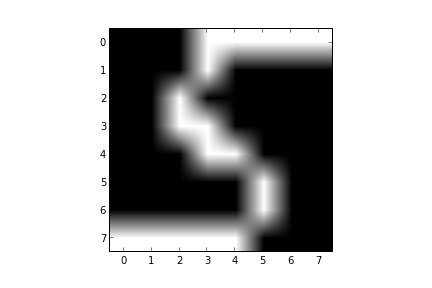
\includegraphics[height=3cm]{boltzmann_01.png}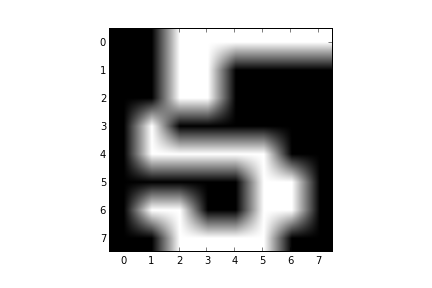
\includegraphics[height=3cm]{boltzmann_02.png}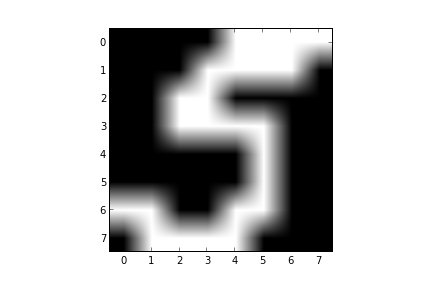
\includegraphics[height=3cm]{boltzmann_03.png}





\begin{minted}[fontsize=\footnotesize]{python}
from pymc import *
X = Uniform('X', zeros(20), ones(20), value=0.5*ones(20))
@pm.potential
def SNLS(X=X):
    logp = -X[0]**2 / X[1]
    logp += -X[1]**2 / X[2]  # or whatever...
    return logp
m = pm.MCMC([X, SNLS])
m.use_step_method(pm.AdaptiveMetropolis, X)
m.sample(100)
print X.trace().sum()
print X.trace()
\end{minted}

\begin{verbatim}
 [-----------------100%-----------------] 100 of 100 complete in 0.0 sec859.644700277
[[ 0.46223878  0.48128005  0.55810033 ...,  0.42273698  0.44134661
   0.58229281]
 [ 0.36116954  0.48722963  0.58007443 ...,  0.46051786  0.32241747
   0.51418611]
 [ 0.35089803  0.4896898   0.47508852 ...,  0.35913589  0.33566267
   0.42208466]
 ..., 
 [ 0.08665662  0.73061874  0.8907893  ...,  0.0650032   0.30217511
   0.74186561]
 [ 0.08665662  0.73061874  0.8907893  ...,  0.0650032   0.30217511
   0.74186561]
 [ 0.08665662  0.73061874  0.8907893  ...,  0.0650032   0.30217511
   0.74186561]]
\end{verbatim}


















Information Theory, Inference and Learning Algorithms

http://nbviewer.ipython.org/gist/aflaxman/7d946762ee99daf739f1


















\end{document}
